
\documentclass[11pt,a4paper]{article}

\usepackage[utf8]{inputenc}
\usepackage[T1]{fontenc}
\usepackage[spanish]{babel}

\usepackage[margin=2.2cm]{geometry}
\usepackage{graphicx}
\usepackage{booktabs}
\usepackage{tabularx}
\usepackage{float}
\usepackage{array}

\usepackage[
    backend=biber,
    style=ieee,
    sorting=none
]{biblatex}

\addbibresource{referencias/sanchez.bib}
\addbibresource{referencias/loor.bib}
\addbibresource{referencias/zambrano.bib}

\title{Notas de la exposición\\
Computación paralela y análisis de RabbitMQ}
\author{Sánchez, Loor y Zambrano}
\date{21 de Noviembre de 2026}

\begin{document}

\maketitle

\section*{Desarrollo de la exposición}

% ============================================================
% Notas de Darwin Sánchez: apartados 1, 2 y 3 (4 minutos)
% ============================================================
\subsection*{Darwin Sánchez: fundamentos, arquitectura y transparencias}

Diez diapositivas en cuatro minutos. El ejemplo es una tienda en línea que
publica sus pedidos en RabbitMQ para que varios trabajadores los procesen.

\begin{table}[H]
\centering
\small
\begin{tabular}{@{}clc@{}}
\toprule
\textbf{N.\textsuperscript{o}} & \textbf{Diapositiva} & \textbf{Tiempo} \\
\midrule
1 & ¿Qué es la computación paralela? & 0:20 \\
2 & Paralelismo, concurrencia y sistemas distribuidos & 0:25 \\
3 & Ejemplo: varios trabajadores procesando pedidos & 0:25 \\
4 & Ejemplo: pedidos de distinta duración & 0:30 \\
5 & RabbitMQ: qué es y qué problema resuelve & 0:25 \\
6 & Usuarios, aplicaciones y escenarios de uso & 0:15 \\
7 & Componentes de la arquitectura & 0:20 \\
8 & Diagrama propio: recorrido de un pedido & 0:35 \\
9 & Transparencias presentes en la arquitectura & 0:25 \\
10 & Limitaciones de esas transparencias & 0:20 \\
\midrule
 & \textbf{Total} & \textbf{4:00} \\
\bottomrule
\end{tabular}
\end{table}

\paragraph{1. Computación paralela.}
Dividir un problema en subtareas que se ejecutan al mismo tiempo en varios
procesadores para terminar antes, coordinando a quienes trabajan. Puede ser
de memoria compartida, distribuida (paso de mensajes) o híbrida
\cite{dai2025parallel}.

\paragraph{2. Paralelismo, concurrencia y sistemas distribuidos.}
Concurrencia: varias tareas avanzan en el mismo período, aunque se turnen;
paralelismo: se ejecutan a la vez \cite{reinders2023}. Un sistema distribuido
son máquinas autónomas que se comunican por red y se ven como uno solo
\cite{vansteen2023distributed}. En la tienda se dan los tres. Los hilos se
ven en el apartado de comunicación.

\paragraph{3. Varios trabajadores.}
Seis pedidos iguales: un trabajador tarda seis turnos; tres trabajadores, dos.
Es el caso ideal. En RabbitMQ basta conectar varios consumidores a la misma
cola \cite{rabbitmq2026amqp}.

\paragraph{4. Pedidos de distinta duración.}
Si P1 y P4 tardan 4 minutos y el resto 1, el reparto por turnos de RabbitMQ
le da los dos grandes al trabajador 1 y todo termina en 8 minutos. Con
\texttt{prefetch} = 1 cada trabajador recibe otro pedido solo tras su
\texttt{ack}, y se termina en 5 \cite{rabbitmq2026workqueues}. No basta con
más trabajadores: importa cómo se reparte. El \texttt{prefetch} reaparece en
el caso Kodus.

\paragraph{5. RabbitMQ.}
Broker de mensajería de código abierto que recibe mensajes de productores y
los entrega a consumidores \cite{rabbitmq2026home,rabbitmq2026amqp}. En la
tienda permite responder sin esperar el procesamiento, no conocer a los
trabajadores y absorber picos de pedidos en la cola \cite{fu2021fair}.

\paragraph{6. Usuarios y escenarios.}
Es uno de los tres brokers principales para aplicaciones web, con Kafka y
Pulsar \cite{dyjach2024brokers}; Kodus es un caso real
\cite{malinosqui2026kodus}. En la tienda lo usamos como cola de trabajo y
para enviar el pedido a dos colas.

\paragraph{7. Componentes.}
La tienda publica por un canal de su conexión TCP en un \textit{exchange}, que
según sus \textit{bindings} decide a qué colas va el mensaje; la cola lo
guarda en orden y los trabajadores lo reciben y confirman
\cite{rabbitmq2026connections,rabbitmq2026channels,rabbitmq2026amqp}.

\paragraph{8. Diagrama.}
Seguir los pasos de la Figura~\ref{fig:arquitectura-rabbitmq}: (1) la tienda
publica con la clave \texttt{pedido.creado}; (2) el \textit{exchange}
\texttt{pedidos} la copia en \texttt{procesar\_pedidos} y
\texttt{notificar\_cliente}; (3) P1, P2 y P3 se procesan a la vez mientras
P4, P5 y P6 esperan; (4) sin \texttt{ack}, el pedido pasa a otro trabajador
\cite{rabbitmq2026queues}. La cola es de quórum, replicada en tres nodos
\cite{rabbitmq2026quorum}.

\begin{figure}[H]
  \centering
  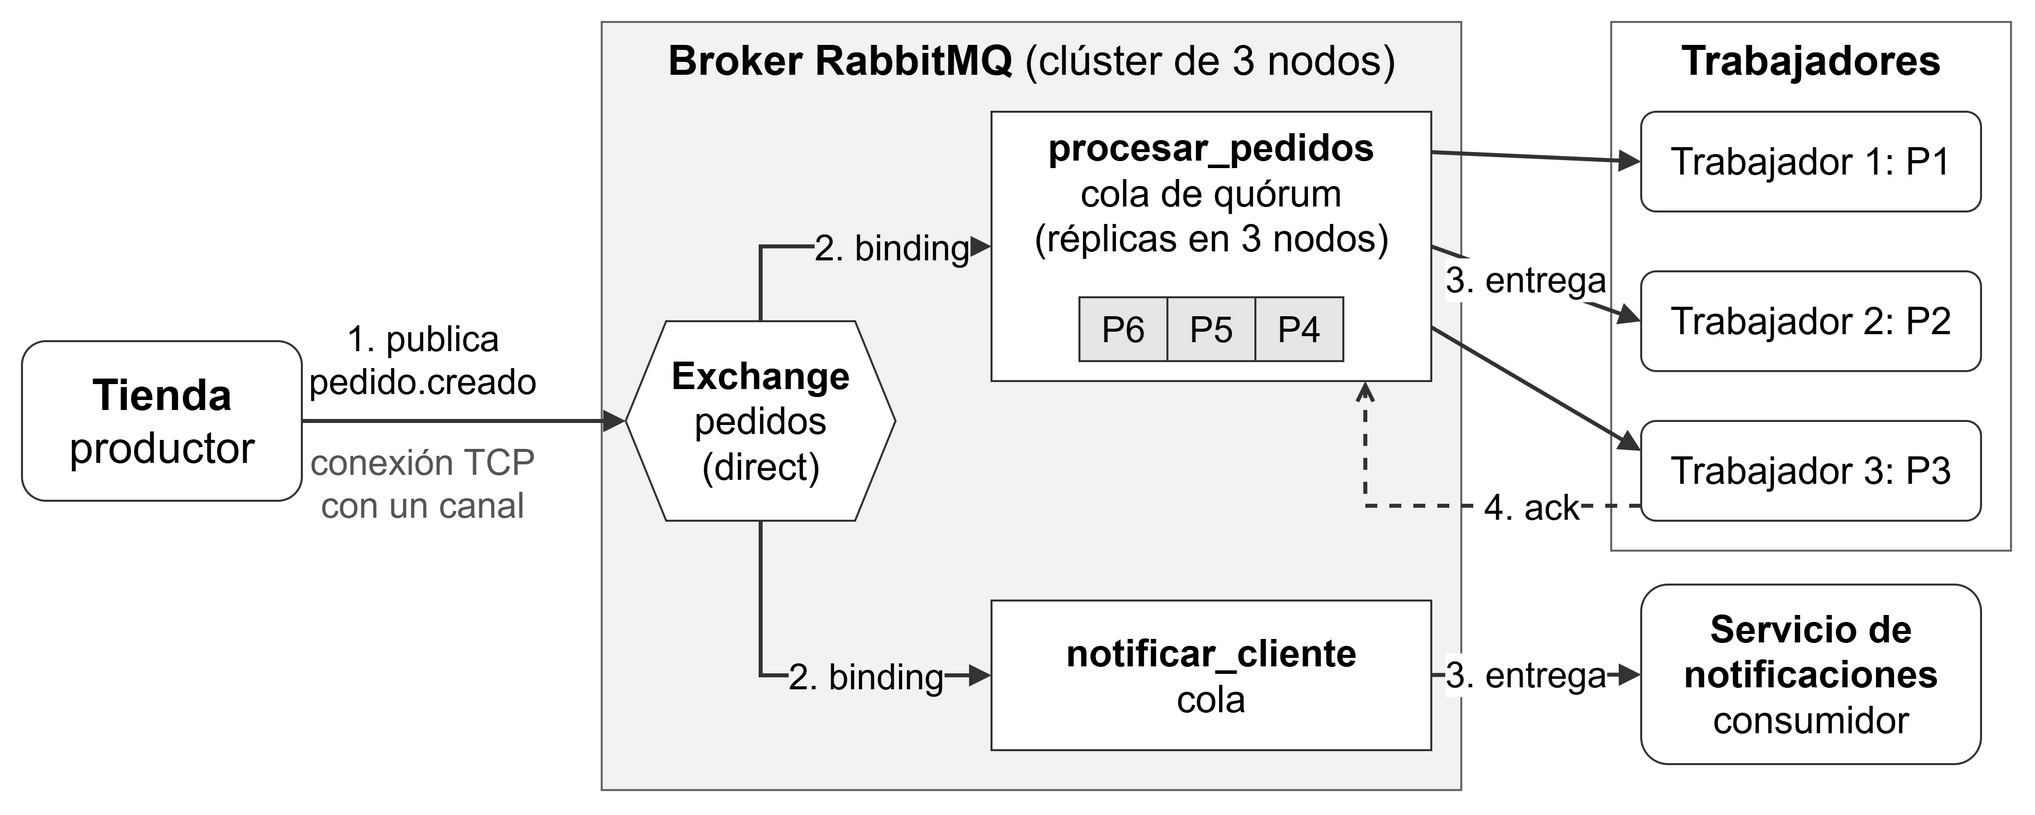
\includegraphics[width=0.85\textwidth]{diagramas/arquitectura.png}
  \caption{Recorrido de un pedido en RabbitMQ. Elaboración propia.}
  \label{fig:arquitectura-rabbitmq}
\end{figure}

\paragraph{9. Transparencias.}
La tienda no sabe qué trabajador ni qué nodo atiende el pedido (ubicación),
la cola replicada se ve como una sola (replicación), los trabajadores la
comparten sin coordinarse (concurrencia) y, si uno cae, su pedido pasa a otro
(fallos) \cite{vansteen2023distributed,rabbitmq2026clustering}.

\paragraph{10. Limitaciones.}
Un pedido reentregado puede procesarse dos veces; si cae un nodo, la tienda
debe reconectarse; con tres nodos la cola de quórum solo tolera un fallo; y la
demora de la red no se oculta \cite{rabbitmq2026queues,rabbitmq2026quorum}.
Estos compromisos se analizan con CAP y PACELC en el apartado siguiente.

% GA-SUM-02 / EXP-1 — Notas del integrante 2 (Steffanny Loor)
% Guion oral aproximado: 4 minutos.
% Citas selectivas a fuentes técnicas; bibliografía compartida en referencias/loor.bib.

\section*{Guion de exposición — Steffanny Loor (4 minutos): comunicación y procesamiento paralelo}

\subsection*{Diapositiva 1. CAP: consistencia, disponibilidad y particiones (30 s)}
CAP nos ayuda a entender qué ocurre cuando se interrumpe la comunicación entre nodos.
Consistencia significa que las lecturas reflejan el estado más reciente;
la disponibilidad, que las solicitudes reciben una respuesta válida;
y tolerancia a particiones, que debemos considerar fallos de red.
 En una quorum queue de RabbitMQ con tres miembros se necesita una mayoría de dos.
 Si uno queda aislado, los otros dos pueden continuar, pero el miembro aislado no puede confirmar publicaciones p
 or su cuenta \cite{ahmed2023,myrhorodskyi2025,rabbitmq2026quorum}.

\subsection*{Diapositiva 2. PACELC (23 s)}
PACELC amplía este análisis.
Durante una partición, debemos considerar el compromiso entre
consistencia y disponibilidad. Incluso cuando la red funciona,
coordinar réplicas puede hacer que aumente la latencia.
En RabbitMQ, las quorum queues utilizan consenso y necesitan una mayoría.
 Por eso, no sería correcto clasificar a todo RabbitMQ de una sola manera:
 depende del tipo de cola y su configuración \cite{ahmed2023,myrhorodskyi2025,rabbitmq2026quorum}.

\subsection*{Diapositiva 3. Diagrama: dos formas de procesar un pedido (25 s)}
Este diagrama compara dos situaciones.
 En la primera, la aplicación espera que termine una
 operación antes de continuar. En la segunda, publica el
 pedido en una cola de RabbitMQ y puede seguir atendiendo s
 solicitudes. Varios consumidores comparten la cola y
 procesan pedidos diferentes. Esto permite distribuir el
 trabajo: si varios consumidores se ejecutan simultáneamente,
 los pedidos pueden procesarse en paralelo \cite{maharjan2023,derlatka2023,reinders2023}.

\subsection*{Diapositiva 4. Comunicación síncrona y asíncrona (12 s)}
La comunicación síncrona espera una respuesta para continuar;
la asíncrona permite avanzar sin esperar el procesamiento
del mensaje \cite{kazanavicius2023}.

\subsection*{Diapositiva 5. Comunicación síncrona (18 s)}
Una tienda necesita conocer si el pago fue aprobado antes de
confirmar la compra. La comunicación síncrona permite tomar
esa decisión, aunque puede introducir demoras \cite{kazanavicius2023}.

\subsection*{Diapositiva 6. Comunicación asíncrona (18 s)}
En la comunicación asíncrona, el emisor envía un mensaje y
no tiene que esperar a que el receptor termine de procesarlo.
Las colas almacenan mensajes pendientes y permiten que los componentes
trabajen en momentos diferentes.
Eso reduce su dependencia temporal, aunque requiere gestionar
los mensajes \cite{maharjan2023,derlatka2023}.

\subsection*{Diapositiva 7. Comparación (15 s)}
La diferencia principal es la espera. La comunicación síncrona
conviene cuando necesitamos una respuesta para decidir qué hacer.
La asíncrona conviene cuando una tarea puede quedar pendiente mientras
la aplicación continúa. Ninguna es mejor en todos los escenarios,
además, ser asíncrono no significa automáticamente ejecutar tareas en paralelo.

\subsection*{Diapositiva 8. Hilos, concurrencia y paralelismo (22 s)}
Un hilo es una unidad de ejecución dentro de un proceso. Hay
concurrencia cuando varias tareas progresan durante un mismo
período, aunque se alternen. Hay paralelismo cuando realmente
se ejecutan al mismo tiempo. Pensemos en tres trabajadores:
si se turnan, hay concurrencia; si trabajan simultáneamente,
hay paralelismo. En RabbitMQ, varios consumidores pueden recibir pedidos distintos;
solo existe paralelismo si los procesan al mismo tiempo. Tener varios consumidores no
lo garantiza por sí solo \cite{reinders2023}.

\subsection*{Diapositiva 9. Modelos de comunicación (20 s)}
En cliente-servidor, un proceso solicita un servicio y otro
lo atiende. En mensajería, los procesos intercambian mensajes,
a veces mediante un intermediario. En RPC, un proceso solicita
ejecutar una operación en otro. RabbitMQ funciona como intermediario
entre productores y consumidores y también permite construir patrones de petición
y respuesta \cite{zhang2023,kazanavicius2023}.

\subsection*{Diapositiva 10. Procesamiento asíncrono con RabbitMQ (18 s)}
En nuestro ejemplo, un cliente realiza un pedido,
la aplicación publica un mensaje y RabbitMQ lo dirige a una
cola. Después, uno de los consumidores recibe y procesa ese pedido.
Otros consumidores pueden atender pedidos distintos. Así, la aplicación
no espera a que cada trabajador termine. Si hay recursos para ejecutar
varios consumidores simultáneamente, diferentes pedidos pueden procesarse en
paralelo \cite{maharjan2023,derlatka2023}.

\subsection*{Diapositiva 11. Aplicación al PFC: SREI (27 s)}
En mi de fin de curso, SREI, en mi grupo tenemos dos servicios independientes
con Spring Boot. El servicio de eventos proporciona información y el
servicio de consulta la solicita mediante REST.
Elegimos comunicación síncrona para esta interacción porque el
consumidor necesita recibir los datos antes de responder a la consulta.
A diferencia del ejemplo de RabbitMQ, aquí no estamos distribuyendo trabajos
pendientes entre consumidores, sino obteniendo una respuesta directa.

\textbf{Fuentes utilizadas:} \cite{ahmed2023,myrhorodskyi2025,rabbitmq2026quorum,kazanavicius2023,maharjan2023,derlatka2023,reinders2023,zhang2023}.
% ============================================================
% Notas de Angel Zambrano: apartados 6, 7 y 8
% ============================================================
\subsection*{Angel Zambrano: fallos, comparación con Kafka y conclusiones}

\paragraph{Tolerancia a fallos.}
Si un trabajador toma un pedido y se cae a mitad del proceso, lo que pase depende de cuándo confirmó. Si espera a terminar para confirmar, RabbitMQ ve que la conexión se cortó y le pasa el pedido a otro trabajador. Para esto usa el \texttt{ack} y \texttt{nack} manual, el prefetch y los \textit{publisher confirms}.

\paragraph{Incidente real: Kodus.}
El 4 de enero Kodus pasó de un solo servidor a tres servicios conectados con RabbitMQ, y recién el 23 de enero dieron con la causa, cuando ya tenían unos 900 \textit{pull requests} en cola. El problema principal fue que RabbitMQ nunca funcionó como clúster por un error en Terraform. Encima el prefetch estaba en 60 y los reintentos por el límite de la API de GitHub dejaban jobs trabados. Corrigieron Terraform, los 900 pedidos salieron en minutos y bajaron el prefetch a 20. Meter más workers no les iba a servir, porque el problema estaba en la configuración \cite{malinosqui2026kodus}.

\paragraph{Comparación con Kafka.}
RabbitMQ funciona como una cola: el mensaje se procesa, se confirma y se borra. Kafka es un registro donde los mensajes quedan guardados y cada consumidor sabe hasta dónde leyó. En Ramadan y otros, RabbitMQ tuvo 4,38 ms contra 83,27 de Kafka con mensajes de 100 KB \cite{rias2026kafka}. En Kamiński, el resultado cambió según la plataforma \cite{kaminski2025rabbitmq}.

\paragraph{Conclusiones.}
Para el SGIRI elegiríamos RabbitMQ, porque lo que movemos son tareas puntuales y el volumen es moderado. Cada aviso se confirmaría con \texttt{ack} manual, el prefetch iría bajo y el que falle varias veces se iría a una cola aparte. Del caso Kodus nos quedamos con revisar que el clúster de verdad esté unido y que los reintentos fallen rápido.


\section*{Tabla de aportes}

\begin{table}[H]
\centering
\small
\begin{tabularx}{\textwidth}{@{}p{2cm}X X@{}}
\toprule
\textbf{Integrante} & \textbf{Responsabilidades} &
\textbf{Evidencias de autoría} \\
\midrule
Sánchez & Fundamentos, arquitectura y transparencias. &
Diagrama, diapositivas, notas y commits propios. \\

Loor & Sincronía, asincronía, hilos, CAP/PACELC y comunicación. &
Diagrama, diapositivas, notas y commits propios. \\

Zambrano & Tolerancia a fallos, comparación y conclusiones. &
Análisis de incidente, diapositivas, notas y commits propios. \\
\bottomrule
\end{tabularx}
\end{table}

\section*{Declaración de uso de inteligencia artificial}

\textbf{Zambrano.} Usé Claude (Anthropic) en mi parte de la exposición. Me
ayudó a buscar artículos con DOI sobre RabbitMQ y Kafka y el post-mortem de
Kodus, que leí y subrayé (capturas en \texttt{evidencias/articulos/}). Claude
redactó la primera versión de las diapositivas de fallos y de comparación, y
armó conmigo el diagrama de causas raíz de Kodus. Las conclusiones las
respondí yo y Claude las pasó a diapositivas. El guion de mis notas lo escribí
yo siguiendo mis diapositivas, y Claude le dio formato \LaTeX{} y agregó las
citas. Revisé que las cifras coincidieran con las fuentes.


\medskip
\noindent\textbf{Steffanny Loor.} Utilicé ChatGPT (OpenAI, GPT-6) en su versión web,
como herramienta de apoyo durante
el desarrollo de mi parte de la exposición.
Me ayudó a comprender conceptos de CAP, PACELC,
comunicación síncrona y asíncrona, concurrencia y
paralelismo. También lo utilicé para revisar la
redacción de las diapositivas, organizar mi guion
de exposición y mejorar el diagrama comparativo
de procesamiento.

Además, utilicé ChatGPT para generar una primera
versión del README del repositorio, que posteriormente
revisé y edité. También me ayudó a dar formato
\LaTeX{} a textos que había escrito previamente.

Comprobé que lo de mi parte compilara y que se generara el pdf
correctamente

\medskip
\noindent\textbf{Ejemplo de prompt utilizado:}
\begin{quote}
``Explica las diferencias entre comunicación síncrona
y asíncrona, concurrencia y paralelismo, utilizando
RabbitMQ como ejemplo de un sistema distribuido.''
\end{quote}

\section*{Bosquejo inicial de arquitectura}


\printbibliography

\end{document}
